\section{Wyniki badań}

\subsection{Wynik badań dla scenariusza 1}

Proces publikacji aplikacji Tabela w repozytoriach oprogramowania Flathub oraz Snap Store został opisany w rozdziale \ref{roz:opis_srodowisk}.

W ocenie autora...


\subsection{Wynik badań dla scenariusza 4}

W tym scenariuszu zbadano czas uruchamiania aplikacji Tabela zainstalowanej za pomocą Flatpak oraz Snap.

%\newpage

\begin{figure}[ht]
    \centering
    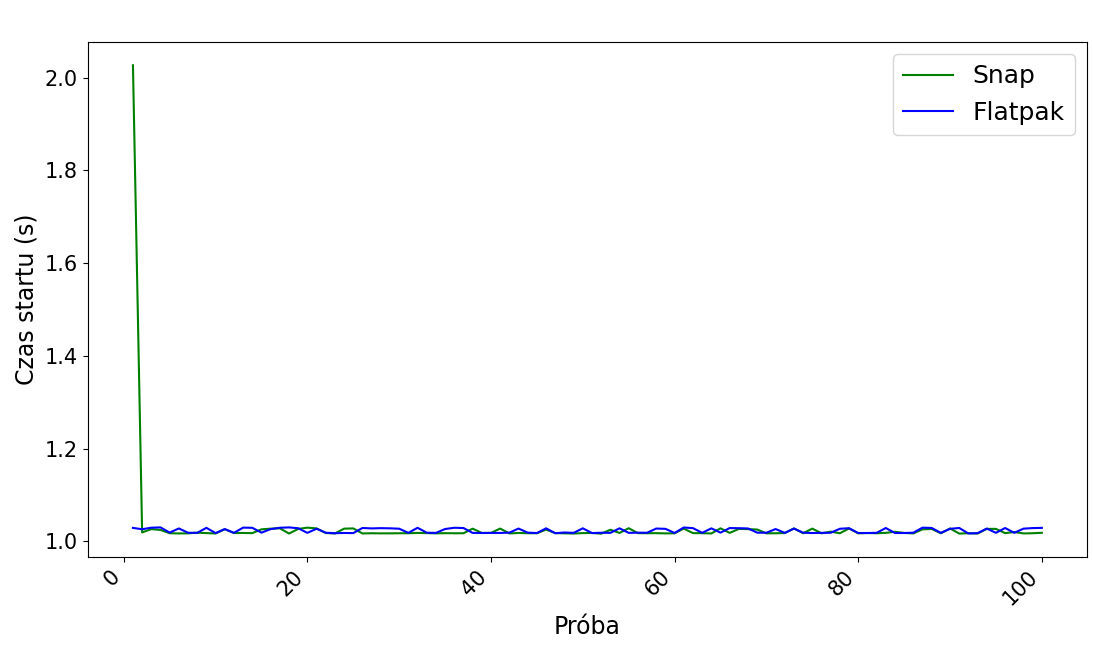
\includegraphics[width=\linewidth]{img/wykresy/czas_wlaczania_4.png}
    \caption{Porównanie czasu uruchamiania aplikacji Tabela w scenariuszu 4}
    \label{wykres:startup}
\end{figure}

Jak wynika z badań wskazanych na rysunku \ref{wykres:startup}, uzyskane...

Narzędzie \cite{hyperfine}...